%%%%%%%%%%%%%%%%%%%%%%% file typeinst.tex %%%%%%%%%%%%%%%%%%%%%%%%%
%
% This is the LaTeX source for the instructions to authors using
% the LaTeX document class 'llncs.cls' for contributions to
% the Lecture Notes in Computer Sciences series.
% http://www.springer.com/lncs       Springer Heidelberg 2006/05/04
%
% It may be used as a template for your own input - copy it
% to a new file with a new name and use it as the basis
% for your article.
%
% NB: the document class 'llncs' has its own and detailed documentation, see
% ftp://ftp.springer.de/data/pubftp/pub/tex/latex/llncs/latex2e/llncsdoc.pdf
%
%%%%%%%%%%%%%%%%%%%%%%%%%%%%%%%%%%%%%%%%%%%%%%%%%%%%%%%%%%%%%%%%%%%

\documentclass[runningheads,a4paper]{llncs}

\usepackage{amssymb}
\usepackage{amsmath}
\setcounter{tocdepth}{3}


\usepackage{graphicx}
\graphicspath{ {images/} }


\usepackage{tabularx}
\newcolumntype{C}{>{\centering\arraybackslash}X}


\bibliographystyle{IEEEtran}

\usepackage{url}
\urldef{\mailsa}\path|{zswanson2, briggan2}@unl.edu|    
\newcommand{\keywords}[1]{\par\addvspace\baselineskip
\noindent\keywordname\enspace\ignorespaces#1}

\begin{document}

\mainmatter  % start of an individual contribution

% first the title is needed
\title{Scalable Vision Transformers \\ for Embedded Systems}

% a short form should be given in case it is too long for the running head
\titlerunning{Scalable Vision Transformers}

% the name(s) of the author(s) follow(s) next
%
% NB: Chinese authors should write their first names(s) in front of
% their surnames. This ensures that the names appear correctly in
% the running heads and the author index.
%
\author{Zachary Swanson \and Benjamin S. Riggan}

%
\authorrunning{Scalable Vision Transformers}
% (feature abused for this document to repeat the title also on left hand pages)

% the affiliations are given next; don't give your e-mail address
% unless you accept that it will be published
\institute{University of Nebraska-Lincoln \\
Department of Electrical \& Computer Engineering,\\
844 N 16th Street, SEC C290, PO Box 880511 \\
Lincoln, NE 68588-0511\\
\mailsa\\
\url{https://engineering.unl.edu/ece/}}

\toctitle{Scalable Vision Transformers}
\tocauthor{}
\maketitle

\begin{abstract}
The abstract should summarize the contents of the paper and should
contain at least 70 and at most 150 words. It should be written using the
\emph{abstract} environment.
\keywords{Vision Transformers, Classification, Edge AI, Optimization}
\end{abstract}

\section{Introduction}
Vision transformers (ViTs) have emerged as an alternative to convolutional neural networks (CNNs) for computer vision, offering unique benefits especially relevant to embedded systems. Unlike CNNs, which extract features hierarchically via localized receptive fields, ViTs treat an image as a sequence of patch tokens and apply self-attention globally. This global receptive field enables ViTs to capture long-range dependencies and holistic context in an image, which can improve robustness on tasks like recognition under significant distortions or at long distances~\cite{rodrigo2024transformersvsCNN}. For example, a transformer can link far-apart parts of an object or face, potentially outperforming CNNs in scenarios where spatial relationships span the entire image. Such ability to model global relationships is advantageous in embedded vision applications like aerial imagery or remote biometric recognition, where important cues may be distributed across the frame.

However, ViTs initially came with drawbacks that pose challenges for resource-constrained devices. Early ViT models were extremely large – the Vision Transformer (ViT) model required hundreds of millions of parameters and pre-training on massive datasets to match CNN accuracy. For instance, the original ViT-Huge had over 600 million parameters and needed extensive training data (e.g. JFT-300M) to outperform CNNs~\cite{dosovitskiy2021vit}. Such high model complexity and memory demands are impractical for embedded devices. Moreover, lacking the built-in inductive biases of CNNs (e.g. translation invariance and locality), vanilla transformers tend to require more data or regularization to generalize well~\cite{dosovitskiy2021vit}. With limited training data, a ViT can struggle to learn stable features, whereas CNNs’ local filtering and weight sharing act as useful constraints. These factors historically limited the adoption of ViTs in edge scenarios.

Despite these challenges, recent research demonstrates that vision transformers can be made efficient and scalable for edge deployment. Data-efficient training techniques and compact architectures have narrowed the gap between ViTs and CNNs on limited data~\cite{touvron2021deit,mehta2022mobilevit}. In fact, properly designed transformer models can now achieve competitive accuracy and runtime on embedded hardware: EfficientFormer-L1 attains 79.2\% ImageNet top-1 accuracy with only 1.6~ms latency on an iPhone 12 (CoreML), matching the speed of a MobileNet-V2 while outperforming it by over 4\% in accuracy~\cite{li2022efficientformer}. This progress overturns the notion that transformers are too heavy for mobile/embedded use. ViTs also offer an architectural flexibility (modular self-attention layers) that is amenable to model compression techniques (pruning, quantization, etc.) and parallel acceleration on modern NPUs~\cite{liu2025survey_vit_edge,ceva2023transformer_npu}. In summary, vision transformers provide powerful global feature modeling and scalability, and ongoing innovations are making them viable for embedded systems. 

This chapter explores the development of ViTs for embedded systems in detail. Section~\ref{sec:anatomy} provides an overview of the ViT architecture including explanations of the core components and descriptions of ViT variants and other models explored in this work. Section~\ref{sec:optim} highlights optimization strategies commonly employed for training transformers including low-rank adaptation (LoRA) and knowledge distillation. Section~\ref{sec:experimental} provides an experimental setup that analyzes performance of the various ViT and CNN models through the lens of a challenging biometrics dataset, TinyFace. The TinyFace dataset features small facial crops, averaging $30 \times 30$ pixels, with distorted facial imagery \cite{cheng2018lowresface}. This dataset was selected because it simulates the type of data that a real-world embedded system may process as part of a surveillance and facial recognition system. Finally, Section~\ref{sec:performance} presents and analyzes the biometric and computational performance metrics produced by the various models and optimization techniques on the TinyFace dataset. These results provide the reader with valuable data and insights for selecting the correct architecture for their application.

\section{Anatomy of Vision Transformers}\label{sec:anatomy}
The ViT architecture in Figure~\ref{fig:vit_arch} depicts two core components – patch and token generation and the transformer encoder. Both are examined in detail in the following subsections with additional exploration of the multi-head attention mechanism within the transformer encoder.

\begin{figure}
    \centering
    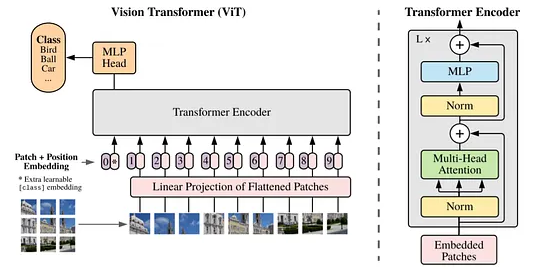
\includegraphics[width=1.0\linewidth]{vit_arch.png}
    \caption{High-level architecture of a Vision Transformer (ViT) from the original ViT paper from Dosovitskiy et al.~\cite{dosovitskiy2021vit}. An input image is divided into fixed-size patches, embedded into tokens, and processed by a stack of transformer encoder blocks composed of multi-head self-attention and feed-forward layers.}
    \label{fig:vit_arch}
\end{figure}

At a high level, the ViT takes a $P \times P$ image and breaks it into $Q \times Q$ patches such that $\left(\frac{P}{Q}\right)^2$ patches are generated, e.g., a $224 \times 224$ image split into $16 \times 16$ patches generates $\left(\frac{224}{16}\right)^2=14^2=196$ patches. These patches are converted into token vectors and fed to the transformer encoder. The encoder performs self-attention between all patches to weight the vectors based on global "importance" and then performs a non-linear transformation via multilayer perceptron (MLP), also referred to as feed forward network (FFN), to generate a new token representation that is fed to the next encoder layer. The encoder process is repeated through multiple encoder layers effectively refining the token representation before delivering the image representation to a task-specific head. This explanation skips over many crucial details that will be presented in the following sections but provides a clear picture of how the image data flows through the transformer model.

\subsection{Self-Attention and Multi-Head Mechanism}
The fundamental component of a transformer is the self-attention layer. In a vision transformer, an image is first split into a sequence of patch embeddings, and a self-attention module then computes interactions between every pair of these patch tokens. Specifically, each token $i$ is projected to a query vector $q_i$, key vector $k_i$, and value vector $v_i$ in some latent dimension. The attention operation compares queries and keys via scaled dot-products: $s_{ij} = q_i \cdot k_j / \sqrt{d}$, where $d$ is the token dimension and is applied to appropriately scale the attention scores. A softmax is then applied to $\{s_{ij}\}$ across all tokens $j$ to obtain attention weights $\alpha_{ij}$, which indicate how much token $i$ attends to token $j$. These weights are used to compute a weighted sum of the value vectors $v_j$ for token $i$, updating its representation. Thus, the full attention operation may be represented as
\begin{equation}
    \text{Attention}(Q,K,V)=\text{softmax}\left(\frac{QK^T}{\sqrt{d_k}}\right)V
\end{equation}
where $Q$, $K$, and $V$ are matrices containing the $q$, $k$, and $v$ vectors for all tokens, respectively. This allows information from one token to directly influence another, regardless of spatial distance, enabling the global receptive field of ViTs~\cite{vaswani2017attention}.

Rather than use a single attention head, some transformers employ multi-head self-attention (MHSA). In MHSA, the token embeddings are projected into multiple subspaces via multiple linear layers (heads), and independent self-attention operations are performed in each subspace in parallel. After performing the parallel attentions, the lower-dimensional tokens are concatenated to produce a token of the same dimension as the original input token. Figure~\ref{fig:multihead_attention} provides an example where three heads are applied to three tokens of length 12, i.e., $d=12$.
\begin{figure}
    \centering
    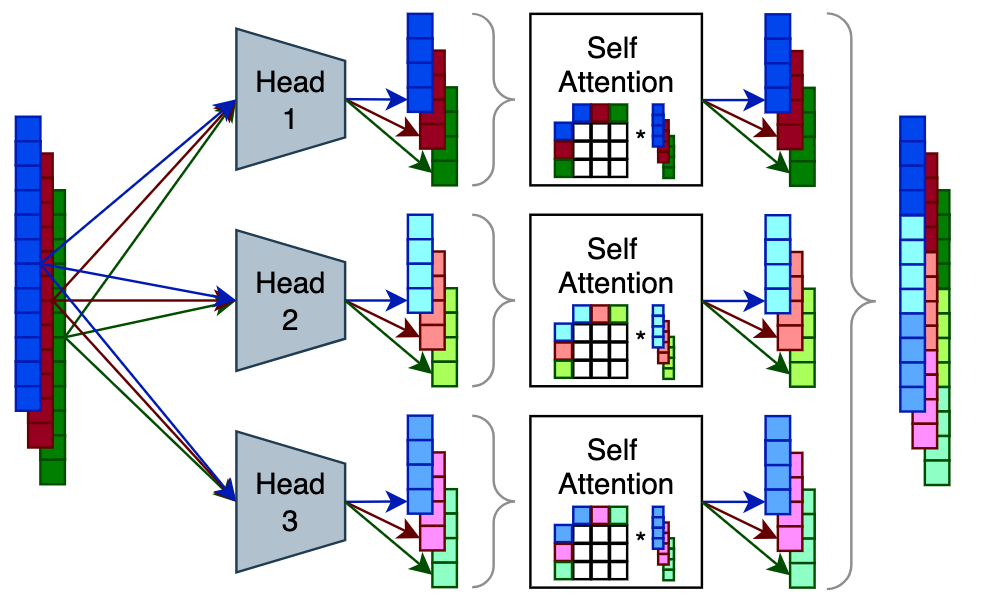
\includegraphics[width=1.0\linewidth]{multihead_attention.png}
    \caption{Example of multi-head self attention on three tokens of length 12 ($d=12$) where each token is passed to three separate linear projection heads to project the tokens to a smaller dimension (4). Thus, each head ideally learns a different representation of the token indicated by the varying shades. Self-attention is performed in parallel for each subspace and the resulting token vectors are concatenated to produce tokens of the same dimensionality as the original.}
    \label{fig:multihead_attention}
\end{figure}

In the example of Figure~\ref{fig:multihead_attention}, three heads are used and each head processes all three tokens of length 12 ($d=12$). Thus, the projected dimension is equal to the original token dimension ($d$) divided by the number of heads ($N_H$) such that $\frac{d}{N_H}=4$, as depicted by the smaller tokens to the right of the heads. The smaller tokens have varying shades of color to indicate that each head learns a different representation of the original token. Then, self-attention is performed independently within each subspace, i.e., there are three self-attention operations performed in this example. The output of the independent attention operations are concatenated to produce tokens with the same dimensionality as the original input token.

This design has two benefits: (1) it allows parallel computation of attention, improving throughput on hardware accelerators by performing many smaller matrix multiplies simultaneously; and (2) each head can learn attention in a different representation subspace, so the model can attend to different kinds of features or relationships in parallel~\cite{vaswani2017attention,zhang2021d2l}. In essence, multi-head attention enables more nuanced and diversified learning, as tokens are compared on distinct portions of their feature descriptors across heads. The outputs of all heads are concatenated and passed through a linear projection to form the final attended representation for each token.

\subsection{Transformer Encoder Structure}
A vision transformer is constructed by stacking multiple \emph{encoder blocks}, each composed of a multi-head self-attention (MHSA) sub-layer followed by a position-wise feed-forward network (FFN), as shown in Figure  ~\ref{fig:vit_arch}. Modern ViT architectures typically adopt a \emph{pre-layer normalization (Pre-LN)} design to improve optimization stability, especially for deep models. In this formulation, layer normalization is applied before both the attention and FFN sub-layers, and each sub-layer output is added to its input via a residual skip connection.

Layer normalization is used in place of batch normalization for several reasons. Unlike batch normalization, which normalizes activations across the batch dimension and therefore depends on batch statistics, layer normalization operates independently on each token by normalizing across feature dimensions. This makes layer normalization well suited to transformer architectures, where inputs are naturally represented as sequences of tokens and batch sizes may be small or variable. In embedded and low-latency settings, small batch sizes are common due to memory constraints, making batch normalization unstable or ineffective. Moreover, layer normalization is invariant to sequence length and batch size, simplifying deployment and enabling consistent behavior during both training and inference~\cite{ba2016layernorm}.

Formally, given an input token sequence $\mathbf{X} \in \mathbb{R}^{N \times D}$, where $N$ is the number of tokens and $D$ is the token length, an encoder block computes
\[
\mathbf{X}' = \mathbf{X} + \mathrm{MHSA}(\mathrm{LN}(\mathbf{X})),
\]
\[
\mathbf{Y} = \mathbf{X}' + \mathrm{FFN}(\mathrm{LN}(\mathbf{X}')),
\]
where $\mathrm{LN}(\cdot)$ denotes layer normalization. This residual formulation preserves gradient flow and enables stable training as depth increases~\cite{he2016resnet}.

The FFN is applied independently to each token and consists of two linear transformations, $W_1$ and $W_2$, with a non-linear activation (commonly GELU), $\sigma$ in between:
\[
\mathrm{FFN}(\mathbf{x}) = W_2 \, \sigma(W_1 \mathbf{x}),
\]
where $W_1$ expands the feature dimension and $W_2$ projects it back to the model dimension. While the MHSA sub-layer performs global information mixing across tokens, the FFN provides local, channel-wise feature transformation~\cite{vaswani2017attention}.

By stacking $L$ such encoder blocks (e.g., $L=12$ or $24$), the model incrementally refines token representations. Earlier layers tend to encode low-level visual patterns and coarse spatial relationships, whereas deeper layers capture higher-level semantic concepts through repeated global attention and nonlinear transformation. This hierarchical abstraction, achieved without explicit convolution, is a defining characteristic of vision transformers and underpins their strong representational capacity~\cite{dorszewski2025concepts_vit}.

\subsection{Tokenization and Position Embeddings}
Before entering the transformer encoder, an input image must be converted into a sequence of tokens. In the standard Vision Transformer (ViT) formulation, this tokenization is performed by partitioning the image into fixed-size, non-overlapping patches (e.g., $16\times16$ pixels) and linearly projecting each flattened patch into a $D$-dimensional embedding space, typically achieved via convolutional layer with stride equal to kernel size. For example, a $224\times224$ image divided into $16\times16$ patches yields $14\times14=196$ patch tokens, each represented as a vector of dimension $D=768$ in a ViT-Base model~\cite{dosovitskiy2021vit}.

In addition to patch tokens, a learnable classification token is commonly prepended to the sequence. This token aggregates global information through self-attention and is used as the image-level representation for classification tasks, following a design originally introduced in BERT~\cite{devlin2019bert} and later adopted for vision transformers. The resulting input to the transformer encoder is therefore a sequence of $N+1$ tokens, where $N$ is the number of image patches.However, this is not a requirement and other architectures like the Swin Transformer~\cite{liu2021swin} perform some method of aggregating all the tokens into a single vector after the final layer.

The self-attention mechanism is permutation-invariant and does not encode spatial order by itself; therefore, positional information must be explicitly injected into the token embeddings. Early transformer models employed fixed sinusoidal positional encodings~\cite{vaswani2017attention}, whereas ViT introduced learned absolute positional embeddings~\cite{dosovitskiy2021vit} that are added to the patch and classification tokens. These embeddings allow the model to associate each token with a specific spatial location in the image grid, enabling meaningful spatial reasoning.

Absolute positional embeddings require special consideration when the input image resolution differs from the pretrained configuration. Since the learned positional embedding table is tied to a fixed number of tokens (e.g., 196 patches for $224\times224$ inputs), changing the image size alters the number and arrangement of patches, resulting in a mismatch between pretrained positional embeddings and the new token grid. To address this, common strategies include interpolating the pretrained positional embeddings to the new spatial resolution or reinitializing and retraining them. While interpolation often works well in practice, it introduces an implicit assumption of spatial smoothness and may slightly degrade performance, particularly when scaling to very small or highly distorted inputs~\cite{ranftl2021dpt,bolya2024window_attention}.

To mitigate these issues, several later architectures replace absolute positional embeddings with relative positional encodings or biases. For example, models such as the Swin Transformer~\cite{liu2021swin} incorporate relative position bias directly into the attention computation, allowing the model to encode spatial relationships between tokens independently of the absolute image size. This design improves generalization to arbitrary resolutions and simplifies deployment across varying input dimensions, which is especially advantageous in embedded and real-world vision systems where input sizes may vary.

\subsection{Architectural Survey of Efficient Vision Models}\label{sec:arch-survey}
The basic ViT described above is often called a “columnar” or non-hierarchical transformer: it processes tokens at one resolution throughout all layers. Furthermore, the original ViT required a significant amount of training data to achieve competitive performance. Numerous architectural variants have been proposed to improve efficiency and performance for vision tasks; a few major variations and CNN baselines relevant to embedded systems are highlighted below.

\paragraph{Data-Efficient Image Transformer (DeiT, 2021):} The DeiT model by Touvron et al. was a crucial step in making transformers practical without massive external data. Architecturally, DeiT is essentially the same as the original ViT (a “base” 12-layer transformer with 86 million parameters) but its innovation lies in the training method. DeiT introduced a knowledge distillation strategy tailored for transformers: a learnable distillation token is appended alongside the class token, and the transformer is trained to predict a teacher CNN’s class logits via this token. By using a pre-trained ResNet as teacher and extensive data augmentation and regularization, DeiT achieved 83.1\% top-1 accuracy on ImageNet using only ImageNet-1k data (no extra pre-training)~\cite{touvron2021deit}. This matches the performance of much larger ViTs that were pre-trained on hundred-million image corpora. The ability to train on a standard dataset with a single GPU machine (in under 3 days) greatly broadened the accessibility of ViTs.

\paragraph{Swin Transformer (2021):} Swin Transformer by Liu et al. is a hierarchical ViT designed as a versatile vision backbone for both image classification and dense tasks. Swin’s key idea is the use of shifted local windows for self-attention. Instead of global attention over all patches, each Swin layer restricts attention to non-overlapping windows (e.g. $7\times7$ patch windows) which drastically reduces computation. To enable cross-window information flow, every other layer the window partitioning is shifted by a certain offset (hence “shifted” windows), so a patch will attend with neighbors that were in different windows in the previous layer. This scheme achieves linear computational complexity in image size (since window size is fixed) while still allowing distant patches to interact after a few layers. Along with this locality, Swin builds a multi-stage pyramid: patch merging layers between stages reduce the number of tokens (by $2\times$ in each spatial dimension) and increase the feature dimensionality, akin to a CNN downsampling. The result is a transformer that behaves much like a CNN feature hierarchy. Swin’s importance is twofold: (1) it significantly lowers memory and compute by limiting attention to local windows, and (2) its multi-scale nature makes it applicable to tasks like detection that are common in embedded vision (e.g. surveillance cameras).

\paragraph{Pyramid Vision Transformer (PVT, 2021):} PVT by Wang et al. was another early effort to adapt transformers as a general-purpose backbone. PVT introduces a pyramid of transformer stages to handle high-resolution inputs efficiently. In PVT, the image is initially patched into a large number of tokens (e.g. $4\times4$ patches) for the first stage, but then at each subsequent stage the tokens are merged (concatenating and projecting patches, similar to pooling) to progressively halve the resolution. This yields a pyramid of feature maps at multiple scales, much like a CNN. By the final stage, the token count is greatly reduced, addressing ViT’s high memory use on large feature maps. Notably, PVT uses full global attention within each stage (no windowing), but because later stages have few tokens, the overall cost remains manageable. The designers also modified the attention to include a spatial reduction on the attention keys/values for further speedup in high-resolution stages. PVT retains the benefit of both worlds: it has the global receptive field of transformers and the pyramidal structure of CNNs~\cite{wang2021pvt}.

\paragraph{MobileViT (2022):} MobileViT by Mehta \& Rastegari is a vision transformer specifically designed for mobile and edge devices. The motivation of MobileViT is to combine the strengths of CNNs and ViTs to create a lightweight model with both local and global feature modeling. The architecture of MobileViT is hybrid: it interleaves convolutional layers with transformer layers in a sequential block. A typical MobileViT block uses a small CNN to extract low-level features, then unfolds those features into a sequence of tokens which are processed by a transformer encoder (attention + FFN), and then folds the tokens back to feature map form which is fused with the convolutional features. This design treats transformers “as convolutions,” effectively inserting a global processing unit within a local CNN context. MobileViT also uses very compact dimensions (e.g. embedding dim 144 or 192) and only a few attention layers, making it comparable in size to mobile CNNs~\cite{mehta2022mobilevit}. MobileViT demonstrates a feasible recipe: use mostly efficient convolutions, but allocate a fraction of computation to MHSA to boost representation power.

\paragraph{ConvNeXt (2022):} ConvNeXt by Liu et al. is a pure convolutional network, included here as a point of comparison because it was directly inspired by the design patterns of transformers. The authors of ConvNeXt asked: if we take a ResNet and modernize it with the tricks that make ViTs successful, can CNNs still compete? They progressively modified a standard ResNet: replacing $3\times3$ convolutions with larger $7\times7$ kernels (to increase receptive field, analogous to global attention), using only depthwise separable convolutions (like a transformer’s factorized attention), moving the location of normalization layers (using layer normalization instead of batch normalization), and increasing network width and depth based on transformer scaling trends. The outcome: ConvNeXt proved to be on par with transformers~\cite{liu2022convnext}. The significance for embedded systems is that CNNs are not obsolete – by adopting transformer-era improvements, CNNs can attain similar accuracy and often with lower inference overhead on certain hardware. Many edge deployments (e.g. DSP or NPU accelerators) are still more optimized for convolutions operations than for MHSA~\cite{Zhao2025H4HNAS,LiPaolieriGolubchik2025,Quadric2023ViT}. ConvNeXt offers a compelling alternative when one needs the best of both worlds: it yields transformer-level accuracy but uses standard convolutions layers that may run more efficiently on existing embedded inference engines. In practice, the choice between ConvNeXt and a ViT may come down to the specific hardware and compiler support. This model underscores that the gap between CNNs and Transformers has narrowed, and both paradigms continue to learn from each other.

\paragraph{ResNet (2016):} Finally, we consider the classical ResNet architecture by He et al. as a baseline. ResNets introduced the concept of residual learning through skip connections, enabling very deep CNNs to train effectively. A ResNet’s computational structure is a chain of convolutional blocks with occasional downsampling, and its strong hierarchical feature extraction made it the dominant vision backbone of the late 2010s~\cite{he2016resnet}. ResNets are relevant to embedded vision as they are highly optimized in many libraries and hardware accelerators; a ResNet-50 can often run in real-time on mobile NPUs after quantization~\cite{ignatov2021ai_benchmark,android2025optimization}. However, compared to newer architectures, ResNets have relatively lower accuracy at a given model size and lack the global attention mechanism of ViTs. Throughout this chapter, we use ResNet variants as a conventional baseline to quantify the improvements delivered by transformer-based models. It’s noteworthy that some efficient ViTs now exceed ResNet-50’s accuracy while being smaller or faster, highlighting the progress in this field.

\section{Optimization Strategies for Embedded Training}\label{sec:optim}
Deploying vision transformers on embedded platforms requires more than efficient architectural design; it also demands training and adaptation strategies that respect constraints on memory, computation, and energy. While most embedded devices are ill-suited for large-scale model optimization, careful separation of offline training and lightweight adaptation enables transformer-based models to be deployed effectively in practice. This section outlines common training pipelines for embedded vision transformers, discusses the trade-offs between offline training and on-device adaptation, and introduces optimization techniques—such as parameter-efficient fine-tuning, knowledge distillation, quantization, and pruning—that facilitate deployment under resource constraints. These strategies form the foundation for the TinyFace case study presented later in this chapter.

\subsection{Training Pipeline and Resource Constraints}
In most real-world scenarios, training large vision transformer models is performed offline on high-performance servers or cloud-based GPUs rather than directly on embedded devices~\cite{mlsys2023ondevice_chapter,ambient2025training_vs_inference}. Vision transformers typically require substantial computational resources, including high memory bandwidth and large batch sizes, to train effectively. Embedded platforms, by contrast, are optimized for inference workloads and generally lack the memory capacity, floating-point throughput, and energy budget required for full model training.

As a result, the dominant training pipeline follows a two-stage approach: models are pretrained or fine-tuned offline using powerful hardware and then deployed to embedded devices exclusively for inference. This paradigm allows developers to exploit advanced optimizers, extensive data augmentation, and long training schedules without imposing additional burdens on the target device. Early embedded machine learning systems largely adhered to this model, focusing on low-latency, on-device inference with pretrained networks~\cite{mlsys2023ondevice_chapter}.

Although on-device training has gained interest due to its potential benefits for privacy, personalization, and domain adaptation, it remains challenging for transformer-based models. Training workloads are significantly more demanding than inference, and even short fine-tuning runs can exhaust memory, increase thermal load, or reduce device lifespan. Consequently, for embedded vision transformers, full training—particularly from scratch—is almost always performed offline, with the device serving as a deployment target rather than a training platform. This separation places greater importance on the robustness and adaptability of the trained model to real-world operating conditions~\cite{lu2025ondevice_training_survey,mlsys2023ondevice_chapter}.

\subsection{Offline Training vs.\ On-Device Adaptation}
While offline training is the preferred approach for developing and optimizing vision transformers, many embedded applications require models to adapt over time to new data, users, or environments. In such cases, a hybrid strategy is often employed in which computationally intensive training is performed offline, while limited adaptation is handled either on-device or through periodic updates from a server.

Offline training offers several advantages, including the ability to use large batch sizes, sophisticated optimization algorithms, and diverse data augmentation strategies. Once trained, models can be compressed through techniques such as quantization or pruning and deployed to embedded devices for efficient inference. When updates are needed, retraining or fine-tuning can be performed offline and redistributed to devices, ensuring consistent performance without incurring on-device training costs.

On-device adaptation, when used, is typically restricted to lightweight updates such as incremental learning of new classes, personalization to user-specific data, or calibration to changing sensor conditions~\cite{nadalini2025odl_tiny,mlsys2023ondevice_chapter}. For example, an embedded camera system may adapt a face recognition model to new identities observed in the field. However, these benefits must be weighed against practical constraints: training even a small subset of parameters can significantly increase energy consumption, reduce responsiveness, and stress limited hardware resources. Furthermore, some optimization techniques and adaptive optimizers are poorly supported on embedded NPUs or DSPs~\cite{mlsys2023ondevice_chapter}.

To balance these trade-offs, techniques such as parameter-efficient fine-tuning, federated learning, and split learning have been explored~\cite{houlsby2019adapter,mlsys2023ondevice_chapter}. These methods aim to minimize on-device computation while preserving adaptability, often by limiting the number of trainable parameters or offloading portions of training to external servers. In practice, offline training remains the primary mechanism for developing embedded vision transformers, while on-device adaptation is applied selectively in scenarios where privacy, personalization, or environmental variability justify the additional resource cost.

\subsection{Parameter-Efficient Tuning (LoRA)}
When adapting large vision transformers to a new task or dataset, updating all model parameters is often unnecessary and computationally expensive. Parameter-efficient fine-tuning (PET) methods address this issue by restricting training to a small subset of parameters while keeping the pretrained backbone fixed. Low-Rank Adaptation (LoRA) is a prominent and effective PET technique that has been successfully applied to vision transformers.

LoRA operates by freezing the original model weights and injecting additional trainable low-rank matrices into selected layers, most commonly the linear projections within multi-head self-attention (MHSA) and, in some cases, the feed-forward networks (FFNs). Rather than updating a full weight matrix $W \in \mathbb{R}^{d \times d}$, LoRA introduces an additive update
\[
W' = W + \Delta W, \quad \Delta W = A B^\top,
\]
where $A \in \mathbb{R}^{d \times r}$ and $B \in \mathbb{R}^{d \times r}$ are trainable matrices of rank $r \ll d$. The original weight $W$ remains frozen, and only the low-rank factors $A$ and $B$ are optimized. Typical rank values such as $r=4$ or $r=8$ introduce only a small fraction of additional parameters while allowing sufficient expressive capacity for task adaptation.

This formulation significantly reduces the number of trainable parameters and associated optimizer state, often to well under $1\%$ of the full model size. Hu et al.~\cite{hu2022lora} demonstrated that LoRA can achieve performance comparable to full fine-tuning across a range of tasks while dramatically lowering training cost. From an optimization standpoint, LoRA also improves stability by constraining updates to a low-dimensional subspace, reducing the risk of overfitting or catastrophic forgetting, as demonstrated in works like PETALface~\cite{narayan2025petalface}.

For embedded and resource-constrained settings, the advantages of LoRA are particularly compelling. Fine-tuning can be performed with smaller batch sizes, reduced memory consumption, and faster convergence, making it feasible to adapt large pretrained models using modest hardware. However, it should be noted that LoRA does not reduce the memory footprint training because all hidden states are required to train the new low-rank matrices~\cite{Wang2025HyCLoRA}. Because the backbone weights remain unchanged, LoRA preserves the model’s original representational capabilities while learning task-specific corrections. In low-resolution face recognition scenarios, for example, LoRA enables a transformer pretrained on high-quality facial imagery to adapt to datasets such as TinyFace without degrading its performance on higher-resolution domains~\cite{narayan2025petalface}. Recent works such as PETALface and FaceMoE~\cite{narayan2025petalface,narayan2024facemoe} further demonstrate that conditioning or gating LoRA updates can improve robustness across varying image qualities, though the underlying low-rank adaptation principle remains broadly applicable.

\subsection{Knowledge Distillation}
Knowledge distillation (KD) is a widely used technique for transferring knowledge from a large, high-capacity \emph{teacher} model to a smaller or more efficient \emph{student} model. Rather than training the student solely on hard class labels, distillation encourages the student to match the teacher’s output distribution, intermediate representations, or both. This process provides additional supervisory signals that can improve convergence, generalization, and sample efficiency, particularly when training compact models.

In the context of vision transformers, knowledge distillation has played a critical role in reducing data and compute requirements. The Data-efficient Image Transformer (DeiT) demonstrated that ViTs could be trained effectively on ImageNet-1k without large-scale pretraining by distilling knowledge from a convolutional neural network teacher. DeiT introduced a learnable \emph{distillation token} alongside the standard classification token, allowing the transformer to explicitly model the teacher’s predictions through an auxiliary supervision path. This design enabled ViTs to achieve competitive accuracy with CNNs while significantly reducing the reliance on massive external datasets~\cite{touvron2021deit}.

Beyond output-level distillation, several works have explored feature-level and attention-level distillation for transformers. In these approaches, the student is encouraged to align intermediate feature maps, attention matrices, or token embeddings with those of the teacher. Such strategies are particularly effective when distilling from a larger transformer into a smaller one, as they transfer structural inductive biases and attention patterns that are not captured by class probabilities alone. For embedded deployment, this enables smaller transformer models to inherit much of the representational power of larger backbones while maintaining lower latency and memory footprints~\cite{zhang2022minivit,wu2022tinyvit}.

From an embedded systems perspective, knowledge distillation is especially attractive because it shifts computational burden entirely to the training phase. The teacher model is used only offline, and the distilled student incurs no additional inference cost. This makes KD complementary to architectural efficiency and parameter-efficient fine-tuning methods such as LoRA. In practice, distillation is often combined with model compression techniques, including quantization or pruning, to further reduce inference cost without significant accuracy degradation.

\subsection{Quantization and Pruning}
In addition to architectural design and training-time optimizations, post-training model compression techniques such as quantization and pruning are essential for deploying vision transformers on embedded platforms. These methods aim to reduce memory footprint, computational cost, and energy consumption while preserving as much predictive performance as possible.

\paragraph{Quantization:}
Quantization reduces the numerical precision of model parameters and activations, typically from 32-bit floating point (FP32) to lower-bit representations such as 16-bit floating point (FP16) or 8-bit integer (INT8). On embedded hardware, lower-precision arithmetic is often significantly faster and more energy-efficient, and it allows models to fit within limited on-chip memory~\cite{Roth2024ResourceEff}. For vision transformers, quantization can be applied to linear projections in attention layers, feed-forward networks, and embedding layers~\cite{Li2023IViT}. Post-training quantization (PTQ) is attractive for deployment because it does not require retraining the model; instead, calibration data is used to estimate appropriate scaling factors~\cite{Shang2024PTQ}. However, transformers can be more sensitive to quantization error than CNNs, particularly in the attention softmax and layer normalization operations~\cite{Ranjan2024MixQViT}. Quantization-aware training (QAT) addresses this issue by simulating quantization effects during training, allowing the model to adapt its parameters to reduced precision~\cite{IBM2023QAT}. In practice, many embedded deployments adopt mixed-precision schemes, retaining higher precision for numerically sensitive operations (e.g., softmax and normalization) while quantizing the bulk of linear layers to INT8. Such hybrid approaches often achieve substantial speedups with minimal accuracy loss~\cite{Lin2022FQViT}.

\paragraph{Pruning:}
Pruning reduces model complexity by removing parameters or structures that contribute little to overall performance. In unstructured pruning, individual weights with small magnitude are set to zero, yielding sparse matrices. While this can significantly reduce parameter count, unstructured sparsity is difficult to exploit on general-purpose hardware without specialized sparse kernels. As a result, structured pruning is often preferred for embedded systems~\cite{Jiang2023SingleShot}.

Structured pruning removes entire components such as attention heads, neurons, channels, or even transformer layers~\cite{Roth2024ResourceEff}. For vision transformers, common strategies include pruning redundant attention heads, reducing the width of feed-forward networks, or dropping entire encoder blocks in deeper layers. Because the transformer encoder is modular and highly repetitive, it lends itself well to such coarse-grained pruning~\cite{Park2023PTPrune}. Importantly, structured pruning produces dense sub-networks that map efficiently onto existing hardware accelerators~\cite{Roth2024ResourceEff}.

\paragraph{Embedded Deployment Considerations:}
From an embedded systems perspective, the effectiveness of quantization and pruning depends strongly on hardware support and software tooling~\cite{Ngo2025EdgeInference}. Many NPUs and DSPs provide native INT8 or mixed-precision acceleration but offer limited support for sparsity\cite{Roth2024ResourceEff}. Consequently, structured pruning combined with quantization-aware training is often the most practical compression strategy for real-world deployment~\cite{liu2025modelcompression,Jiang2023SingleShot}. When carefully applied, these techniques enable vision transformers to meet strict latency, memory, and power constraints while retaining much of their original representational strength~\cite{Li2023IViT}.

\section{Experimental Setup}\label{sec:experimental}
This section describes the dataset, preprocessing choices, training protocol, and evaluation methodology used to assess the performance and deployability of vision transformer models in an embedded setting. The experimental design emphasizes both biometric accuracy and computational efficiency, reflecting the dual objectives of recognition performance and practical deployment.

\subsection{Dataset Selection: TinyFace}
The TinyFace dataset was selected as the primary benchmark for this study due to its emphasis on extremely low-resolution facial imagery. TinyFace contains over 160,000 face images spanning 5,139 identities, with an average native resolution of approximately $30\times30$ pixels. Images exhibit significant degradation due to limited spatial resolution, compression artifacts, pose variation, and illumination changes. These characteristics make TinyFace a particularly challenging dataset for face recognition and a strong proxy for embedded vision scenarios such as long-range surveillance, low-bandwidth sensing, and resource-constrained edge devices~\cite{cheng2018lowresface}.

Unlike many standard face recognition benchmarks that assume high-quality facial crops, TinyFace stresses a model’s ability to extract discriminative features from minimal visual information. This aligns well with the goals of this work, which seeks to evaluate whether scalable vision transformers can remain effective when both input resolution and deployment hardware are severely constrained.

\subsection{Image Resolution and Preprocessing}
All TinyFace images were resized to a fixed spatial resolution of $96\times96$ pixels prior to being passed to the models. This resolution was chosen as a compromise between preserving spatial detail and avoiding excessive upsampling of the original low-resolution images. Given an average native resolution of approximately $30\times30$ pixels, more aggressive resizing (e.g., $112\times112$ or $224\times224$) was found to introduce substantial interpolation artifacts without meaningful gains in discriminative information.

From a transformer perspective, a $96\times96$ input resolution provides a sufficient number of patch tokens to enable effective self-attention while keeping computational cost manageable. For example, with a patch size of $16\times16$, this resolution yields $6\times6=36$ tokens, striking a balance between spatial expressiveness and efficiency. This choice also aligns with embedded deployment goals, where minimizing token count directly reduces attention complexity and memory usage.

\subsection{Training Protocol and Hyperparameter Selection}

\begin{table}[]
    \centering
    \begin{tabularx}{\textwidth}{X|C|C|C|C|C|C} \hline
         & \multicolumn{2}{c|}{Base} & \multicolumn{2}{c|}{Small} & \multicolumn{2}{c}{Tiny} \\ \hline
         & Params & Layers & Params & Layers & Params & Layers \\ \hline
         ConvNeXT  & 87.6 & & 49.5 & & 27.8 & \\
         DeiT-3    & 85.8 & & 38.3 & & 21.7 & \\
         MobileViT &   -  & &   -  & & 17.4 & \\
         PVT       & 81.4 & & 44.7 & & 24.8 & \\
         ResNet    & 62.6 & & 42.5 & & 23.5 & \\
         Swin      & 86.7 & & 48.8 & & 27.5 & \\ \hline         
    \end{tabularx}
    \caption{Caption}
    \label{tab:arch-specs}
\end{table}

Prior to final training runs, hyperparameter sweeps were conducted to identify stable and effective configurations for each model family. These sweeps explored learning rate, batch size, optimizer parameters, and regularization settings, with the goal of identifying hyperparameter regions that produced consistent convergence rather than single-point optima.

Following hyperparameter selection, all models were trained for a fixed duration of 50 epochs on the TinyFace training split. Training was performed offline on GPU hardware, and all models were evaluated using a standard gallery–probe protocol, consistent with common practice in face recognition. In this setup, a gallery set containing one or more reference images per identity is used for enrollment, and probe images are matched against the gallery to assess recognition performance. Rank-based identification metrics were used to quantify accuracy.

\subsection{Model Selection and Optimization Studies}
Based on initial training results, the top-performing architectures were selected for further investigation. These models were used to study the effects of various optimization and compression techniques, including parameter-efficient fine-tuning via LoRA, knowledge distillation, post-training quantization, and structured pruning. Each technique was evaluated in isolation and, where appropriate, in combination to assess its impact on both recognition accuracy and computational efficiency.

\subsection{Embedded Deployment and Performance Evaluation}
To evaluate real-world deployability, all selected models were benchmarked on an NVIDIA Jetson Orin Nano embedded platform. Computational performance metrics included inference latency, throughput, and memory usage, measured under realistic deployment conditions. By pairing biometric evaluation with on-device performance measurements, the experimental setup enables a holistic assessment of accuracy–efficiency trade-offs and provides practical guidance for deploying vision transformers on embedded systems.

Overall, this experimental framework is designed to systematically evaluate how architectural choices and optimization strategies affect both recognition performance and embedded feasibility when operating on extremely low-resolution visual data.

\section{Performance Analysis}\label{sec:performance}

\section{Conclusion}

\bibliography{references}
\end{document}
